\documentclass[border=5pt]{standalone}
\usepackage{tikz}
\usepackage{amsmath}
\begin{document}
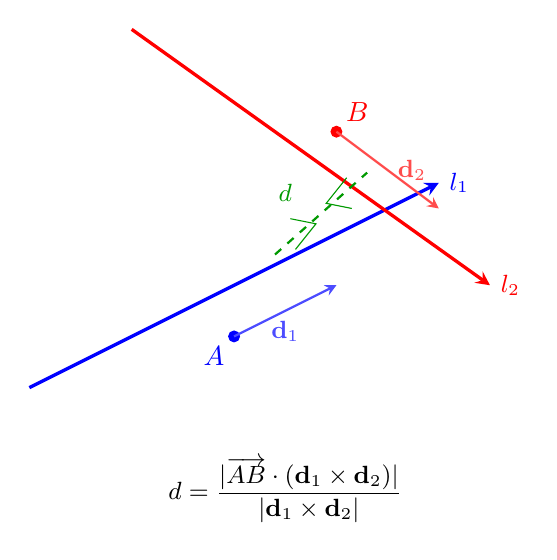
\begin{tikzpicture}[scale=1.3, >=stealth]
  % Distance between two skew lines

  % Line 1
  \draw[very thick, blue, ->] (-2, -0.5) -- (2, 1.5) node[right, font=\small] {$l_1$};
  \filldraw[blue] (0, 0) circle (1.5pt) node[below left] {$A$};

  % Line 2 (skew - not parallel, not intersecting)
  \draw[very thick, red, ->] (-1, 3) -- (2.5, 0.5) node[right, font=\small] {$l_2$};
  \filldraw[red] (1, 2) circle (1.5pt) node[above right] {$B$};

  % Common perpendicular (shortest distance)
  \draw[thick, green!60!black, dashed] (0.4, 0.8) -- (1.3, 1.6);
  \node[green!60!black, font=\small] at (0.5, 1.4) {$d$};

  % Right angle markers
  \draw[green!60!black, thin] (0.6, 0.85) -- (0.8, 1.1) -- (0.55, 1.15);
  \draw[green!60!black, thin] (1.1, 1.55) -- (0.9, 1.3) -- (1.15, 1.25);

  % Direction vectors
  \draw[->, thick, blue!70] (0, 0) -- (1, 0.5) node[midway, below, font=\small] {$\mathbf{d}_1$};
  \draw[->, thick, red!70] (1, 2) -- (2, 1.25) node[midway, right, font=\small] {$\mathbf{d}_2$};

  % Formula
  \node[font=\small] at (0.5, -1.5) {$d = \dfrac{|\overrightarrow{AB}\cdot(\mathbf{d}_1\times\mathbf{d}_2)|}{|\mathbf{d}_1\times\mathbf{d}_2|}$};
\end{tikzpicture}
\end{document}
